% Metódy inžinierskej práce

\documentclass[10pt,oneside,slovak,a4paper]{article}

\usepackage[slovak]{babel}
%\usepackage[T1]{fontenc}
\usepackage[IL2]{fontenc} % lepšia sadzba písmena Ľ než v T1
\usepackage[utf8]{inputenc}
\usepackage{graphicx}
\usepackage{url} % príkaz \url na formátovanie URL
\usepackage{hyperref} % odkazy v texte budú aktívne (pri niektorých triedach dokumentov spôsobuje posun textu)

\usepackage{cite}
%\usepackage{times}
\usepackage{indentfirst}

\usepackage{multicol}
\usepackage{lipsum}

\title{Knižnica ešportu\thanks{Semestrálny projekt v predmete Metódy inžinierskej práce, ak. rok 2022/23, vedenie: Ing. Vladimír Mlynarovič, PhD.}} % meno a priezvisko vyučujúceho na cvičeniach

\author{Matej Kočík\\[2pt]
	{\small Slovenská technická univerzita v Bratislave}\\
	{\small Fakulta informatiky a informačných technológií}\\
	{\small \texttt{xkocikm@stuba.sk}}
	}

\date{\small 6. november 2022} % upravte



\begin{document}

\maketitle

\begin{abstract}
%\ldots 

E-športy sú novovytvárajúcim sa odvetvím športu. V tejto práci si obzrejmíme históriu e-športu~\ref{historia} , ktorá siaha do blízkej minulosti. Predmetom nášho skúmania bude aj hráčska terminológia~\ref{slovnik}, ktorú zahŕňajú najpoužívanejšie pojmy a otázka, či je e-šport naozaj druhom športu~\ref{esportakosport} . 

Chceli by sme predstaviť slovník hráčskeho slangu. Slová vyskytujúce sa v tomto slovníku samozrejme závisia aj od typu hier~\ref{hry} . To znamená, že zväčša každá hra má osobitné výrazy, ktoré hráči počas jej hrania používajú. 

V neposlednom rade sa budeme venovať i konkrétnym, najpopulárnejším hrám~\ref{hry} , ich pravidlám a najznámejším hráčom~\ref{klasifikacia:rozdelenie} . Na záver sa budeme zaoberať medzinárodnými turnajmi v jednotlivých hrách~\ref{hry} . Cieľom článku je oboznámiť čitateľa so základnými princípmi, slovami, históriou ešportu ako aj zostaviť slovník výrazov z hráčskeho sveta.
\end{abstract}



\section{Úvod}

%\\

Nová doba, nové informácie, nové inovácie. V technologickom priemysle ku koncu dvadsiateho storočia nastal oborvský ošiaľ v rámci počítačov. Boli spístupnené širokej verejnosti a spočiatku nepredstaviteľná predstava sa transformovala do skutočnosti. V spojení s vynájdením internetu, ľudsko zaznamenalo najväčší technologický pokrok v histórii. Práve to otvorilo pomyselnú bránu neobmedzených možností~\ref{historia} . Ľudia odjakživa fantazírovali a vytvárali si predstavy o nereálnom svete čo je v dnešnom pomímaní zadefinované ako virtuálna realita. Rapídny pokrok spôsobil vytváranie prvotných hier až po také grafické zdokonalenie hier ako ich poznáme dnes. Vývoj hier a gaming samozrejme priniesol svoje negatíva, ale i pozitíva. E-šport sa vytváral ruka v ruke s počítačmi, internetom a všeobecne online svetom. E-športy strhli masy ľudí a stali sa hlavným zdrojom zábavy, oddychu…\cite{a1}


\section{Stručná história elektronického športu} \label{historia}

Prvý turnaj sa podľa dostupných informácií konal na Stamfordskej univerzite. Výhercom Spacewar bolo udelené ročné predplatné časopisu Rolling Stones. Jedným z prvých turnajov, ktoré zaujali nie len obrovské množstvo hráčov, ale aj divákov bol turnaj v hre Space Invaders v roku 1980.

Najväčší ošiaľ so sebou priniesla herná konzola Atari 2600. Významne sa pričinila o presun hráčskeho priestoru z herien do pohodlia domova. Existovala aj zdokonalená verzia tejto konzole, ktorá stála v tom čase približne dve tisíc amerických dolárov. Walter Day založil prvý hráčsky tím v roku 1983. Bol vášnivým priekopníkom hier a pokorovaní rekordov v miestnych herňách a práve toto hobby ho doviedlo vytvoriť Americký národný videoherný tím.  

90. roky sa vyznačovali najmä FPS(First person shooter – pohľad strelca z prvej osoby) hrami. Nosným bodom bolo, že FPS hry sa ovládali pomocou počítača a myši, čo bolo medzi hráčmi veľmi obľúbené. Spomedzi všetkých hier vytŕčali najmä RTS(Real time strategy) hry. Ďalším dôležitým milníkom je vytváranie online serverov, ktoré hráčom umožňovali súťažiť proti ostatným hráčom v globálnom merítku. Kto však prístup k internetu a online serverom nemal, mohol navštíviť internetové kaviarne, ktoré poznáme aj dnes. Veľké množstvo peňazí sa nalialo do e-športu najmä v roku 1997. Výherca turnaju si mohol prilepšiť o čiastky v desať tisícoch dolárov. \cite{a1}


\section{Klasifikácia ešportu} \label{klasifikacia}

\subsection{Definícia ešportu a jeho štruktúra} \label{klasifikacia:definicia}

Ešport alebo elektronický šport je pojem pre súťažné hranie počítačových alebo konzolových hier. Hlavným cieľom ešportu je organizovať súťaže v rôznych hrách ako aj vytváraním organizácií, tímov a zjednocovaním hráčov po celom svete. Spočiatku sa hranie hier – gaming považoval iba za akúsi voľnočasovú aktivitu. Neskôr prišiel pojem ešport, ktorý zmenil pohľad ľudí a spoločnosti na túto oblasť a začal sa klásť do profesionálnej roviny.\cite{a3}

\subsection{Najznámejšie organizácie a tímy} \label{klasifikacia:organizacie}

Hráčske organizácie majú pod sebou profesionálnych hráčov a každá sa samostatne zameriava na určitý typ hry. Ich hlavnou úlohou je pre hráčov vytvoriť čo najpohodlnejšie, najpríjemnejšie a najlepšie prostredie pre rozvoj ich schopností. Podporujú hráčov finančne ako aj po stránke sponzoringu ich herného vybavenia. 

Profesionáli musia mať čo najvýkonnejšie a najrýchlejšie počítače, myšky prispôsobené ich preferencii ako aj kvalitný monitor až po veci, ktoré spadajú do zdravotnej sféry. Poznáme samozrejme aj organizácie jednotlivcov ako napríklad v hre Hearthstone – každý hráč reprezentuje sám seba ako jednu organizáciu. V našich končinách zatiaľ nemáme profesionálny tím, ktorý by našu krajinu mohol reprezentovať na medzinárodnej svetovej úrovni.\cite{a4} Najznámejšími organizáciami sú: FaZe Clan(CS:GO, PUBG, Call of duty, FIFA, Fortnite), OpTic Gaming(Valorant, Call of duty, Overwatch), G2 Esports(Valorant, CS:GO, LOL…), Natus Vincere(CS:GO, FIFA, Fortnite, LOL, Valorant, PUBG).\cite{a5}

\begin{figure} [h!]
 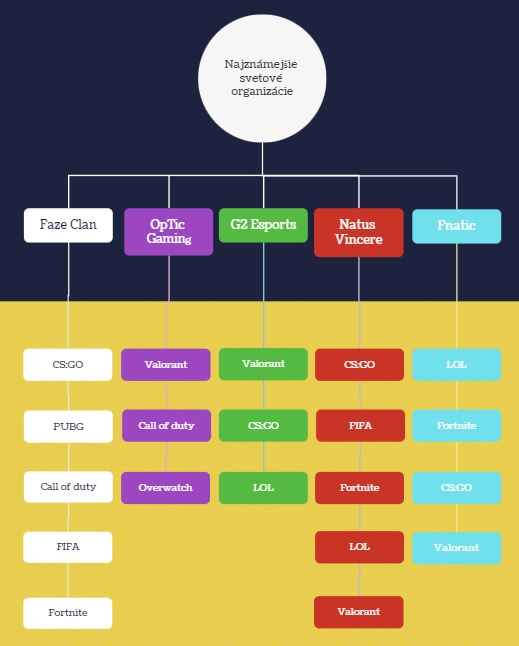
\includegraphics[scale=0.86]{Hráčske organizácie a hry.jpg}
 \caption{Diagram najznámejších hráčskych organizácií a týmov podľa hier, \newline
 Zdroj: \cite{a5}, obrázok: vlastná práca autora}
\end{figure}



\subsection{Rozdelenie hráčov, streameri, influenceri} \label{klasifikacia:rozdelenie}

Každý šport má svoje určité špecifiká, ktoré ich definuje a dáva mu určitú dôležitosť. V klasickom športe poznáme delenie hráčov na amatérskych a profesionálnych. Rozdiel nie je ani v ešporte. Ako súčasť športu sa hráči počítačových hier rovnako rozdeľujú ako pri klasickom športe. Jedinou indifernetnou skupinou sú v ešportoch poloprofesionálni hráči. 
Skupina amatérov a poloprofesionálov za svoje výsledky, výhry nedostáva nijaké peňažné ohodnotenie. Sú to najmä vášnivý hráči, ktorým organizácia zabezpečuje čo najlepšie podmienky pre trénovanie a vybavenie. Je im poskytnutá finančná čiastka na cestovanie na turnaj. 

Profesionáli s organizáciou podpisujú zmluvu. Aké podmienky majú amatéri a poloprofesionáli take isté sú vytvorené pre profesionálov, ale samozrejme vo väčšej miere. Znamená to, že okrem najlepšieho vybavenia majú profesionálni hráči aj finančné ohodnotenie. Profesionáli sú viazaní zmluvou na “full-time job”.\cite{a1}

Množstvo hráčov začalo so streamovaním a následne sa tvrdým tréningom dostali na úroveň profesionálov. Medzi najznámejších slovenských hráčov patrí Ladislav Kovács alias GuardiaN. Je profesionálnym hráčom hry Counter-Strike: Global Offensive(CS:GO)~\ref{hry:csgo} . Túto hru hrával od jej prvej verzie Counter-Strike 1.6, cez neskoršiu verziu Counter-Strike Source, až po aktuálnu verziu Counter-Strike: Global Offensive~\ref{hry:csgo} . Súťažil za najznámejšie svetové tími v CS:GO ako napr. Virtus.pro, Natus Vincere, FaZe clan. Jeho najväčším úspechom bolo umiestnenie na druhom mieste na svete v roku 2015.

Ďalším priekopníkom hry CS:GO je DEV1 vlastným menom Ivan Lazarov. Aktuálne sa už neživí ako profesionálny hráč, ale ako streamer a komentátor turnajov. Je 3-násobným majstrom Českej republiky a jedným z najznámejších osobností herného sveta.\cite{a6}

Kvalitná dobrá propagácia, reclama musí zaujať divákov. Každý streamer a influencer má svoje charakterové črty, ku ktorým diváci vzhliadajú. Sú pre divákov unikátny a zaujímavý. Preto hlavným cieľom organizácií vyhľadať streamerov a influencerov s čo najväčším možným dosahom. Títo známi ľudia propagovajú nejaký turnaj, súťaž, aby bola pre divákov čo najzaujímavejšie vykreslená.\cite{a1}


%\paragraph{Veľmi dôležitá poznámka.}
%Niekedy je potrebné nadpisom označiť odsek. Text pokračuje hneď za nadpisom.


\section{Hráčska terminológia} \label{slovnik}


\begin{multicols}{2}

\end{multicols}


\begin{multicols}{2}
\begin{enumerate}

\item ACE
\begin{itemize}
 \item Hra: CS:GO ~\ref{hry:csgo}
 \item Použitie: používa sa ak 1 hráč zabije celý nepriateľský tým
\cite{a1}
\end{itemize}

\item ADAPT
\begin{itemize}
 \item Hra: Hearthstone
 \item Použitie: efekt, ktorý vylepšuje miniona
\cite{a1}
\end{itemize}

\item AFK
\begin{itemize}
 \item Význam: Preč od klávesnice
 \item Hra: všetky
 \item Použitie: univerzálne – ak si hráč musí odskočiť = nemôže hrať 
\cite{a1}
\end{itemize}

\item BAN
\begin{itemize}
 \item Význam: zamrazenie účtu od adminov
 \item Hra: všetky
 \item Použitie: univerzálne – ak hráč nedodržiava pravidlá hry alebo serveru
\cite{a1}
\end{itemize}

\item BOT
\begin{itemize}
 \item Význam: postava, ktorá je ovládaná umelou intelligenciou
 \item Hra: všetky
 \item Použitie: univerzálne – ak je v hre alebo na serveri nedostatočný počet hráčov, alebo niekto prestane hrať
\cite{a1}
\end{itemize}

\item CLANTAG
\begin{itemize}
 \item Význam: klanové označenie
 \item Hra: všetky
 \item Použitie: do profilu hráča je možné zapísať sa do nejakého klanu/týmu
\cite{a1}
\end{itemize}

\item CROSSHAIR
\begin{itemize}
 \item Význam: zameriavač
 \item Hra: Strieľačky – CS:GO, Fortnite… ~\ref{hry:csgo}
 \item Použitie: nachádza sa v strede obrazovky a pomáha hráčom lepšie a rýchlejšie zamerať cieľ
\cite{a1}
\end{itemize}
 
\item DROP
\begin{itemize}
 \item Význam: hodiť na zem
 \item Hra: CS:GO, Fortnite, PUBG ~\ref{hry:csgo}
 \item Použitie: ak ma niekto vela peňazí v hre tak môže spoluhráčovi kúpiť zbraň a hodiť mu ju
\cite{a1}
\end{itemize}

\item ECO
\begin{itemize}
 \item Hra: CS:GO ~\ref{hry:csgo}
 \item Použitie: nijaký hráč z týmu nič nekupuje, hraje iba s pištoľom, s ktorým sa začína hra
\cite{a1}
\end{itemize}

\item FPS
\begin{itemize}
 \item Význam: snímky za sekundu
 \item Hra: všetky
 \item Použitie: čím väčší je počet FPS tým je hra plynulejšia 
\cite{a1}
\end{itemize}
 
.
\item HERO POWER
\begin{itemize}
 \item Význam: hrdinova sila
 \item Hra: Hearthstone
 \item Použitie: každý hrdina ju má a môže ju použiť ak má 2 many.
\cite{a1}
\end{itemize}

\item NERF
\begin{itemize}
 \item Význam: oslabenie
 \item Hra: všetky
 \item Použitie: ak vývojári oslabia postavu alebo zbraň v hre 
\cite{a1}
\end{itemize}
\end{enumerate}
\end{multicols}

%\newpage

\section{Najpopulárnejšie hry, najlepší hráči a veľké turnaje} \label{hry} 

\subsection{Counter-Strike: Global Offensive} \label{hry:csgo}

Counter-Strike: Global Offensive je bezpochybne jednou z najznámejších, najpopulárnejších a najhranejších hier na svete. CS:GO je kompetitívna multiplayer FPS hra. Je to tímová hra, ktorá sa hraje štýlovm 5 hráčov(1. tím) proti 5 hráčom(2. tím). Dve predošlé verzie boli Conter-Strike 1.6 a Counter-Strike: Source. Je veľmi obľúbená najmä medzi mladými dospievajúcimi ľuďmi. Pôvodne sa hrala na 16 výherných kôl, čo stále platí pre súťažnú formu, však rokmi aktualizácií a vylepšení priniesli v súčaasnej dobe aj formát Wingman a skrátené kompetitívne zápasy na 9 víťazných kôl. Wingman je kompetitivný zápas, na ktorom sa zúčasťňujú dva tímy s dvoma hráčmi na každej strane. Poznáme dva tábory – tábor teroristov(T site) a tabor counter-teroristov(CT site). Táto hra sa hrá na 16 víťazných kôl. Po uplynutí polovice vypísaných kôl si tímy menia strany.\cite{a1}

Hlavným cieľom teroristického táboru je dostať sa na jedno z dvoch miest na mape, označených písmenami A a B, a následne na jedno z nich položiť, aktivovať bombu. Nastavený časový limit na položenie bomby sú dve minúty. No tu práca teroristov ešte nekončí, práve začína. Najťažšou časťou hry pre teroristov je ubránenie bomby pred CT respektíve udržanie bomby aktívnej pokiaľ nevybuchne. Teroristický arzenál je odlišný od toho Counter-teroristického. V inventári s anachádzajú zbrane ako AK-47, Glock, SG 550… Je dôležité spomenúť, že zbrane sú v reálnom svete naozaj vyrábané. Každý prototyp je teda nadizajzovaný podľa skutočnej predlohy. Hoci je väčšina zbraní odlišných, sú aj take, ktoré sa zhodujú pre oba tímy. Napr. AWP, pistol Desert Eagle alebo IMI Negev.\cite{a1}

Na strane obrancov stoja counter-teroristi. Obidve strany si vyžadujú vytvorenie nejakej stratégie respektíve taktiky na dosiahnutie cieľa a splnenie svojej úlohy. Omylom nie je ak povieme, že si tábor counter-teroristov musí určiť viac premyslenejšiu taktiku. Ich úlohou je správne a efektívne pokryť pozície na miestach s označením A a B na uloženie bomby. Ak sa im nepodarí eliminovať teroristický tím, ktorý aktivuje bombu v tom prípade ju musia CT do časového limitu explózie zneškodniť. Ich inventár zbraní pripomína arzenál ozbrojených síl, špeciálnych bojových jednotiek…\cite{a1} 

Na začiatku každého kola si môže hráč v krátkom čase vybrať nejakú zbraň, čo závisí od jeho finančného stavu(peniaze sa získavajú na základe vyhratého/prehratého kola). Máp v hre CS:GO je mnoho, ale najhranejšími I používanými mapami na turnajoch sú: Dust II(vojnou zničené mesto v juhozápadnej Ázii), Inferno(talianske sedliacke mestečko), Mirage(vojnou zničené mesto), Overpass(budovy, parky, základne), Train(vlakové depo).\cite{a1}


\subsection{League of Legends} \label{hry:lol}

Hra je známa aj pod skratkou LOL. Hráč si strategicky veberá postavu (dostupnú zo šampiónov) a snaží sa spoločne so spoluhráčmi zničiť NEXUS. Je to stavba na druhej strane mapy pri spawne hráčov nepriateľského týmu. 

Šampióni sa počas hry môžu vylepšovať, ale začínajú iba s jednou schopnosťou. Dokopy ich je 148 a každý z nich má jedinečnú unikátnu schopnosť. Výherným týmom sa stane ten, ktorý zničí všetky veže chrániace NEXUS a aj NEXUS samotný. \cite{a1}

\subsection{FIFA} \label{hry:fifa}

FIFA je športová hra, ale zároveň aj meno najväčšej svetovej organizácie futbalu. Každý rok sa priaznivci môžu tešiť na novú verziu, ktorá je označená aj rokom respektíve sezónou(napr. FIFA 22). Hráči ju nájdu na všetkých patmormách – počítače, herné konzoly… 

Pravidlá hry sú rovnaké ako pri klasickom futbale, ktorý poznáme. Tvárou hry je vždy iný futbalista, a všetci futbalisti, ligy, organizácie, ktoré sú stvárnené v hre sú licensované. 

Hra obsahuje aj vicero herných módov ako vlastnú kariéru(vytvorenie si vlastného týmu, nákup hráčov, financovanie, liga, pohárové súťaže…), multiplayer mód, pri ktorom je možné si zahrať s druhým človekom a samozrejme aj single player mód. \cite{a1}

\newpage
\section{Záver} \label{zaver} % prípadne iný variant názvu

Tento šport je rýchlo narastajúci na popularite na celom svete. Svet potrebuje určitú virtuálnu formu zábavy a už si bez nej svet nevieme ani predstaviť. Vždy však treba dbať aj na to, abz sa táto záľuba – koníček nepretransformovali do formy závislosti. Každým rokom čím ďalej tým viac narastajú čísla v počte strávených hodín pri hraní hier. Táto tabuľka to len potvrdzuje. Preto sa treba snažiť uvoľniť sa, ale vždz so zdravou mierou. Jednoznačne sa smer ešportu bude len a len vyvíjať a posúvať dopredua už nikdy nezanikne. 

\begin{center}
\begin{tabular}{||c c||} 
 \hline
 Krajina & Čas strávený hraním hier za týždeň v hodinách \\ [0.8ex] 
 \hline\hline
 Veľká Británia & 13,3 \\ 
 \hline
 Nemecko & 9,5\\
 \hline
 Francúzsko & 9,2 \\
 \hline
 Španielsko &  9,2 \\
 \hline
 Taliansko & 8,5 \\ 
 \hline
Priemer & 9,94 \\ [1ex] 
 \hline
\end{tabular}
 %\caption{Zdroj: vlastná práca autora}
\newline Zdroj: \cite{a7}
\end{center}
%\acknowledgement{Ak niekomu chcete poďakovať\ldots}




% týmto sa generuje zoznam literatúry z obsahu súboru literatura.bib podľa toho, na čo sa v článku odkazujete
\bibliography{literatura}
\bibliographystyle{plain} % prípadne alpha, abbrv alebo hociktorý iný

\newpage
\title{PREDNÁŠKY - témy}
\maketitle\newline

\title{SWOT analýza}
\maketitle\newline

Táto téma ma zaujala predovšetkým z dôvodu, že už som so SWOT analýzou prišiel do kontaktu. Jednou spoločnou vecou všetkých úspešných ľudí, ktorých môžeme vidieť v televízii či na internete je, že všetci si uvedomili svoje silné stránky respektíve svoje prednosti a začali ich rozvíjať, aby im to neskôr prinieslo úžitok. Či je to už pracovitosť, dravosť, komunikatívnosť, ambicióznosť… Čo je ešte dôležitejšie, múdry človek sa zakaždým poučí z chýb najmä iných. K tomuto všetkému nás má viesť práve SWOT analýza. Mala by byť akýmsi zrkadlom a uvedomením si vlastných nedostatkov, ale aj predností. Špeciálnou vecou je, že tu sa človek sámm pred sebou neskryje ani sa neoklame. Ak áno, tak oklame len sám seba a v konečnom dôsledku sa nikde neposunie. Silné stránky, slabé stránky, ohrozenia, príležitosti – 4 základné sekcie SWOT. Ak si ich spíšeme a budeme to takto robiť v nejakých pravidelných časových intervaloch tak vtedy sa naozaj vieme pozrieť na to či napredujeme, alebo len stagnujeme.\newline


\title{Vplyv počítačov na zdravie}
\maketitle\newline

Zdravie. Téma, ktorá tu bola odjakživa. Je prirodzené, že príchodov nových technických vymožeností sa svet zameral aj na zdravie v tomto prostredí. Najdiskutovanejšou témou je jednoznačne elektro-magnetické žiarenie. Je veľmi nebezpečné, pretože ľudia ho nijako nepociťujú na svojom tele, čo je však realitou je, že z mobilných vysielačov alebo mikrovlnnýh rúr elektro-magnetické žiarenie vyžaruje. Dnes o vplyve na nás o tom nevieme veľmi vela pretože vedecká spoločnosť sa v názoroch líši. V neposlednom rade sú problémom najmä ochorenia chrbtice, ktoré idú ruka v ruke s poruchou zraku alebo problémy s rukami. Zdravie je jedinečné a pre každého človeka by malo bzť čo najcennejšie a vždy sa človek snaží vymyslieť niečo čo by prípadným problémom predchádzalo ako napr. ergonomické stoličky prispôsobené pre správne držanie tela počas sedenia. Veľkou nevýhodou je, že väčšina týchto vecí sa z finančného hľadiska k obyčajnjému človeku nedostanú. Je však potrebné si zdravie čo najviac chrániť a najmä pri elktronických zariadeniach.\newline

\title{Prezentovanie a komunikačné schopnosti}
\maketitle\newline

Dnešný svet si vyžaduje vela. Tie najväčšie korporácie a inštitúcie si vyhľadávajú najlepších z najlepších. Jednou z hlavných predností je určite aj komunikácia a ako sa tomu v angličtine hovorí tkz. "soft skills". Ak sa chce dnešný človek niekam dostať vždy potrebuje či už zamestnávateľa, alebo zamestnanca presvedčiť a mať vysoko vyvinuté komunikačné schopnosti. Myslím si, že výučba a celkovo prístup ku prezentovaniu respektíve royprávaniu, agitovaniu, presvedčovaniu by sa mali posilniť. Škola nie je prvým miestom, kde sa s ňou človek stretne, ale škola by mala byť miestom, kde si jednolivec môže svoje “soft skills” posilňiť. Vplyvom rapídneho technologického pokroku v posledných rokoch sa ľudia čoraz častejšie zatvárajú do svojich úkrytov virtuálneho sveta a preto často vidíme akúsi neschopnosť komunikovať, či prezentovať svoje myšlienky, názory, postrehy.Je naozaj veľmi dôležité správne prezentovanie seba najmä v tom najlepšom svelte pre lepšiu budúcnosť. Myslím si, že prezentovať a komunikovať sa môže naučiť každý, len potrebuje mať správneho učiteľa.

\end{document}
